\chapter{Natural Image Matting }
\label{chap:natural-image-matting}

\section{Introduction to matting}
\label{sec:introduction-to-matting}

A basic formulation that compositing is based on \cite{compositing} can be defined as follows: given the foreground colour \textit{F=\(F_r,F_b,F_g\)}, the background colour \textit{B=\(B_r,B_b,B_g\)} and $\alpha$, for each pixel the compositing operation is defined by \textit{C=$\alpha$F+(1-$\alpha$)B}. The \textit{RGBA} quadruple for the foreground pixels to be composited, with first three values the colour channels and the fourth value the alpha channel, can be represented for example as \textit{(1,0,0,1)} for an opaque red pixel, \textit{(0,0,1,0.5)} for a blue semi-transparent pixel or \textit{(0,1,0,0)} for a green transparent pixel. So, taking as an example the second case the compositing equation (\ref{eq:composite_e_e}) could be solved as:

\begin{equation} \label{eq:composite_e_e}
\begin{split}
F=(0,0,0),\;B=(0,0,1),\;\alpha=0.5,\;C=?,\\
C_r=0,\;C_g=0,\;C_b=0.5 \times 0+(1-0.5) \times 1\;
\Rightarrow\;C_g=0.5,\\
C=(0,0,0.5)
\end{split}
\end{equation}

So by compositing a black foreground pixel with a blue background pixel and by using a semi–transparent alpha value for the foreground, the resulting pixel in the composite is basically a dark blue pixel.
\par
Matting is the inverse problem; assume that you have an image that is composited with foreground \textit{F} and background \textit{B}. Given an image colour \textit{C}, find \textit{F}, \textit{B} and \textit{$\alpha$} so \textit{C=$\alpha$F+(1-$\alpha$)B} is valid. Since \textit{F} or \textit{B} distinct values aren’t prior known, the equation has multiple solutions. In \textit{Blue Screen Matting} \cite{blue} the image is given and the background colour is known (\textit{chroma key}). So assuming that the foreground does not have chroma key colours within it, eliminating chroma key values from the equations i.e. setting them to zero, will produce the foreground. This is the most extensively used method in films, since the background of a scene can be easily set to a single colour (Figure 2).

\begin{figure}[t!]
%\centering
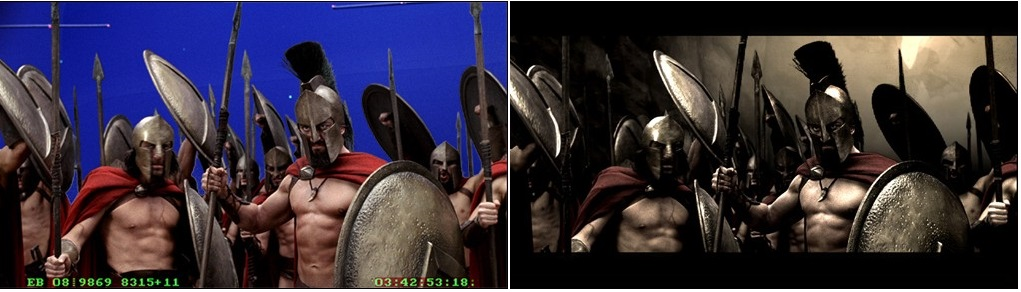
\includegraphics[width=1\columnwidth]{Chapter2/2/bluescreen.jpg}
\caption[Blue screen used in the movie 300.]{Blue screen used in the movie 300. The film was shot using the digital backlot technique, where the whole movie shooting took place in front of blue backgrounds.}
\label{fig:bluescreen}
\end{figure}

Another approach is having two images with the same foreground but different backgrounds, assuming that the two images are completely aligned. In this case the \textit{triangulation} method is used by creating a matrix with six equations and four unknowns and the solution of it gives the \textit{RGB} and $\alpha$ values for the foreground pixels \cite{blue}. The triangulation method is typically used for still images since it would not be practical for film purposes. 
In natural image matting we have an image \textit{I} or composite \textit{C} but no knowledge of foreground \textit{F} and background \textit{B} components. As mentioned in the previous chapter this is an under constrained problem and prior information must be used. 

%%%%%%%%%%%%%%%%%%%%%%%%%%%%%%%%%%%%%%%%%%%%%%%%%%%%%%%%%%%%%%%%%%%%%%%%
\section{Bayesian matting}
\label{sec:bayesian-matting}

In 2001 a research team including well-known computer vision researcher Szeliski, attempted to solve the natural image matting problem using a Bayesian framework \cite{bayesian}. The idea is that given an image \textit{C}, for each pixel find the foreground, background and alpha values that maximize the probability of observing the pixel’s colour (\ref{eq:bayesian_e_a}). Using Bayes rule (\ref{eq:bayesian_e_b}), we have the following formulation:

\begin{subequations}\label{eq:bayesian_e}
\begin{equation}\label{eq:bayesian_e_a}
arg\;\underset{F,B,a}{max}\;P(F,B,\alpha\mid C)
\end{equation}
\begin{equation}\label{eq:bayesian_e_b}
= arg\;\underset{F,B,a}{max}\;P(C\mid F,B,\alpha)P(F)P(B)P(\alpha)/P(C)
\end{equation}
\begin{equation}\label{eq:bayesian_e_c}
= arg\;\underset{F,B,a}{max}\;L(C\mid F,B,\alpha)+L(F)+L(B)+L(\alpha)
\end{equation}
\end{subequations}

Notice that the probability of the image is disregarded since it is constant and doesn’t affect any of the other terms (\ref{eq:bayesian_e_c}). Also F, B and $\alpha$ terms are treated independently and the problem is then expressed as a sum of log probabilities (\ref{eq:bayesian_e_c}). The first term is considered the data term and is modelled with (\ref{eq:bayesian_e_2}), and the other terms are the prior probabilities and are modelled via (\ref{eq:bayesian_e_3}).

\begin{equation} \label{eq:bayesian_e_2}
L(C\mid F,B,\alpha)=-\left \| C-\alpha F-(1-\alpha)B \right \|^{2}/\sigma_{C}^{2}
\end{equation}

\begin{equation} \label{eq:bayesian_e_3}
L(F)=-(F-\overline{F})^{T}\Sigma _{F}^{-1}(F-\overline{F})/2
\end{equation}

In (\ref{eq:bayesian_e_2}) sigma is a tunable parameter and in (\ref{eq:bayesian_e_3}) the covariance matrix and mean can be computed by samples collected based on the trimap. \textit{F} is substituted by \textit{B} to get the log likelihoods of background and $\alpha$ likelihood is initially considered to be constant. Figure 3 is a visualization of the idea.

\begin{figure}[t!]
%\centering
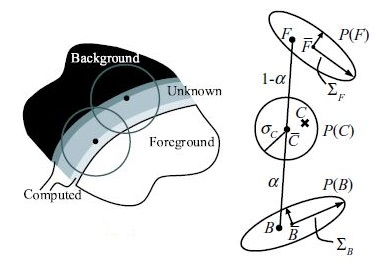
\includegraphics[width=0.5\columnwidth]{Chapter2/2/bayesian_figure_1.jpg}
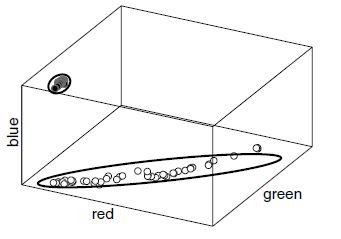
\includegraphics[width=0.5\columnwidth]{Chapter2/2/bayesian_figure_2.jpg}
\caption[Foreground and background distributions.]{Trimap (left) with corresponding distributions (middle). Distributions of foreground and background colours in RBG colour space are fitted within ellipses (right). Figures taken from \cite{bayesian} and \cite{visualeffects}.}
\label{fig:bayesian_e_f_4}
\end{figure}

By substituting the equations (\ref{eq:bayesian_e_2}) and (\ref{eq:bayesian_e_3}) and solving them by taking partial derivatives,\textit{ F} and \textit{B} are estimated assuming that $\alpha$ is constant. On the other hand, assuming that \textit{F} and \textit{B} are constant, (\ref{eq:bayesian_e_4}) is used to estimate $\alpha$. The two methods are alternated until estimated \textit{F}, \textit{B} and $\alpha$ converge.

\begin{equation} \label{eq:bayesian_e_4}
\alpha =\frac{(\textbf{C}-\textbf{B})\cdot (\textbf{F}-\textbf{B}))}{\left \| \textbf{F}-\textbf{B} \right \|^{2}}
\end{equation}

The problem that arises from this formulation is that modelling colour distributions in natural images cannot be done with a simple probability density function, because in natural images the distributions will possibly be overlapping. A proposed solution is to model the distributions as a mixture of Gaussian distributions (Figure 4).

\begin{figure}[t!]
\centering
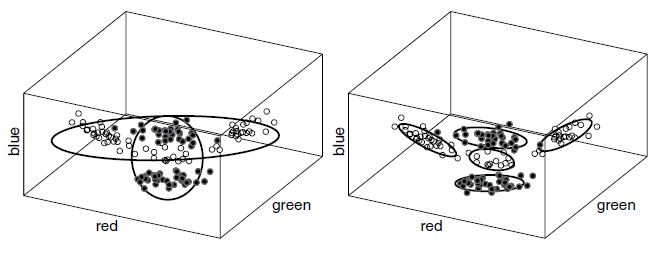
\includegraphics[width=0.8\columnwidth]{Chapter2/2/bayesian_figure_3.jpg}
\caption[Overlapping distributions.]{Overlapping F and B colour distributions (left). F and B colour distributions fitted into multiple ellipses (right). Figure taken from \cite{visualeffects}.}
\label{fig:bayesian_figure_3}
\end{figure}

%%%%%%%%%%%%%%%%%%%%%%%%%%%%%%%%%%%%%%%%%%%%%%%%%%%%%%%%%%%%%%%%%%%%%%%%%%%%%%%%%%%%%%%%%%%%
\section{Closed Form matting}
\label{sec:closed-form-matting}

Another major contribution to solving the matting problem was introduced in 2008 by Levin et al \cite{closedform} where an observation made in natural images lead to the assumption that within a small window around a pixel, pixel values in \textit{RGB} colour space lie on straight lines. This idea is called the \textit{colour line model} and can be visually represented in Figure 5a. If \textit{$C_{i}$} is a colour pixel and \textit{$B_{0}$} is a background pixel within a colour line, $\alpha_{i}$ can be estimated by (\ref{eq:closed-form-e1}). $\alpha_{k}$ is the vector connecting the foreground and background colour lines (Figure 5c).

\begin{equation}\label{eq:closed-form-e1}
\alpha_{i}=\textbf{$\alpha_{k}$}\cdot (\textbf C_{i}-\textbf B_{0})= \alpha _{k} \cdot \textbf{C}+b_{k}
\end{equation}

\begin{figure}[t!]
\centering
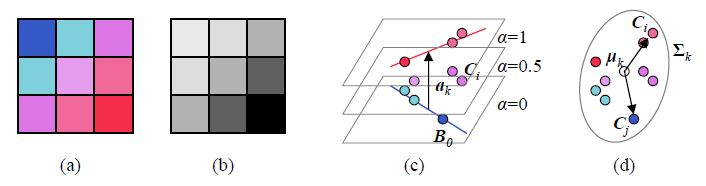
\includegraphics[width=1\columnwidth]{Chapter2/2/closed_form_figure_1.jpg}
\caption[Colour line model and alpha superposition.]{Colour line model and alpha superposition. A 3x3 window in an image with colour values (a) and intensity values (b). The pixels fitted to colour lines in RBG space and the superposition of a (c). Figure taken from \cite{algorithmsapplications}.}
\label{fig:closed-form-f1}
\end{figure}

A cost minimization function for all estimated a values over all windows is formulated in (\ref{eq:closed-form-e2}) where $\epsilon$ is a regularization term for overlapping distributions. For each window the energy function is simplified leading to (\ref{eq:closed-form-e3}), where \textit{L} is the \textit{Laplacian matrix} or \textit{matting Laplacian} and can be determined by (\ref{eq:closed-form-e4}); $\delta_{i,j}$ is the Kronecker delta, \textit{M} is the number of pixels in each (overlapping) window, \textit{$\mu_{k}$} is the mean colour of the pixels in window \textit{$W_{k}$}, and \textit{$\Sigma_{k}$} is the 3x3 covariance of the pixel colours (Figure 5d).

\begin{equation} \label{eq:closed-form-e2}
E_{\alpha}=\sum_{k}(\sum_{i\in W_{k}}(\alpha_{i}-\alpha_{k}\cdot C_{i}-b_{k})^2)+\epsilon\left \| \alpha_{k} \right \|)
\end{equation}

\begin{equation} \label{eq:closed-form-e3}
E_{\alpha}=\alpha^T\textbf{L}\alpha
\end{equation}

\begin{equation} \label{eq:closed-form-e4}
L_{ij}=\sum _{k:(i,j)\in W_{k}}(\delta _{ij}-\frac{1}{M}(1+(C_{i}-\mu _{k})^T\hat\Sigma_k ^{-1}(C_{j}-\mu _{k})))
\end{equation}

The user provided scribbles for definite foreground and definite background pixels, provide the energy function some prior a values, so only a sparse set of linear equations has to be solved. When $\alpha$’s are calculated, the foreground and background colours are estimated using a least squares minimization of the compositing equation regularized with a spatially varying first order smoothness (\ref{eq:closed-form-e5}). $\lambda\left |\bigtriangledown \alpha_{i}  \right |$ weights separately the x and y components of the F and B derivatives.


\begin{equation} \label{eq:closed-form-e5}
E_{B,F}=\sum _{i}\left \| C_{i}-[\alpha+F_{i}+(1-a_{i})B_{i}] \right \|^{2}+\lambda\left |\bigtriangledown \alpha_{i}  \right |(\left \| \bigtriangledown F_i \right \|^{2}+\left \| \bigtriangledown B_{i} \right \|^2)
\end{equation}

Another observation made by the authors, was that even before user information about the image was provided, the \textit{eigenvectors} of the matting Laplacian corresponding to the smallest \textit{eigenvalues}, reveal a surprising amount of information about potentially good mattes. They subsequently proposed an algorithm called \textit{Spectral matting} \cite{spectral} were the \textit{K} smallest eigenvectors are used as matting components to form a full matte (Figure 6).

\begin{figure}[t!]
\centering
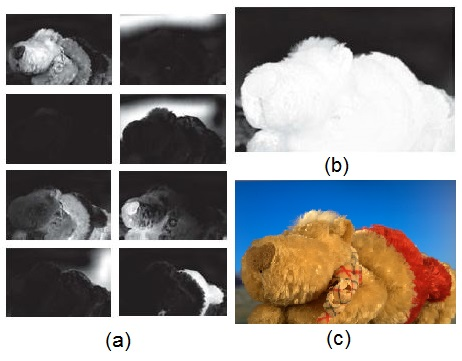
\includegraphics[width=0.8\columnwidth]{Chapter2/2/closed_form_figure_2.jpg}
\caption[Eigenvector images.]{In Spectral matting the eigenvectors that correspond to the smallest eigenvalues (a) can be used as matte components. The combination of them leads to a full matte (b) when compared to the image (c). Figure taken from \cite{spectral}.}
\label{fig:closed-form-f2}
\end{figure}

%%%%%%%%%%%%%%%%%%%%%%%%%%%%%%%%%%%%%%%%%%%%%%%%%%%%%%%%%%%%%%%%%%%%%%%%%%%%%%%%%%%%%%%%%%5
\section{Other matting methods}
\label{sec:other-matting-methods}

Although Bayesian and Closed Form matting had shown promising results, they were still struggling for highly transparent images or images with similar foreground and background colours. The fact that they were well formulated though, gave path for other methods to be developed. Besides using a probabilistic framework or a matting Laplacian, researchers took methods used in other computer vision areas and tailored them for the matting problem. 
An interesting approach is the use of the \textit{gradient} of the image in a method called \textit{Poisson matting} \cite{poisson}. First the spatial gradient of the matting equation is taken (\ref{eq:poisson-1}), typically in the intensity channel of the image, and if the foreground and background are relatively smooth compared to $\alpha$ i.e. $\alpha\bigtriangledown F+(1-\alpha)\bigtriangledown B$ is close to 0, the matte gradient will be proportional to the image gradient and the matte gradient can be approximated by (\ref{eq:poisson-2}). 

\begin{equation} \label{eq:poisson-1}
\bigtriangledown I=(F-B)\bigtriangledown \alpha+\alpha\bigtriangledown F+(1-\alpha)\bigtriangledown B
\end{equation}

\begin{equation} \label{eq:poisson-2}
\bigtriangledown \alpha\approx \frac{1}{F-B}\bigtriangledown I
\end{equation}

This formulation gives a differential equation for $\alpha$ in the unknown region and the minimization of it using information from the trimap, is the same as solving a \textit{Poisson equation} with the same boundary conditions. This method works well with images where background and foreground are both smooth but fails when an image foreground or background has strong gradients.
\par
Wang and Cohen \cite{iterativeoptimization} observed the issue with highly transparent images and the problems caused by a trimap with large unknown regions, so they proposed a \textit{belief propagation} method to determine alpha values. Pixels are marked and grouped. The initial marked pixels are the ones provided by the user as scribbles. Gaussian mixture models are computed for foreground and background pixels that are marked. Then for all pixels that are unmarked: a spatial distance transform is applied to a number of marked pixels and the closest unmarked pixels are marked. A \textit{Marcov Random field} is built based on marked pixels and for each node within it, samples from foreground and background colours are taken and the data cost is computed. Then the belief propagation algorithm is used to estimate a matte for the pixels in the graph and the uncertainty and the estimated foreground and background colours for each pixels in the graph are updated. The marked pixels group is also updated. Experimental results showed a better performance in highly transparent images when using scribbles combined with this method rather than a trimap (Figure 7).

\begin{figure}[t!]
\centering
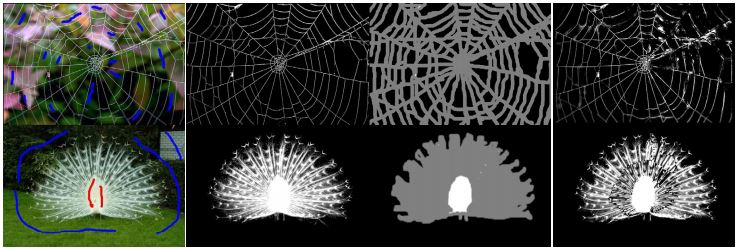
\includegraphics[width=1\columnwidth]{Chapter2/2/2_4_figure_1.jpg}
\caption[Iterative optimization matting results.]{Image alpha mattes are calculated using scribbles and trimaps using the \textit{Iterative Optimization} matting method. Using belief propagation, scribbles produce a better results for images with high transparency. Figure taken from \cite{iterativeoptimization}.}
\label{fig:iterative-optimization-f}
\end{figure}

The same authors a few years later proposed another method \cite{robust} that analysed the confidence of sampled pixels. Assuming that a trimap is provided, for each pixel in the unknown region a number of samples from foreground and background is taken as candidates for estimating foreground and background colours. From the candidates, good samples are considered the ones that as pairs of foreground and background pixels explain the mixed foreground background pixels as linear combinations. A \textit{distance ratio R} is defined (\ref{eq:robust-1}) between sampled pairs and the pixel that is examined, where lower is better. 

\begin{equation} \label{eq:robust-1}
R_{d}(F,B)=\frac{\left \| C-(\alpha F+(1-\alpha)B) \right \|}{\left \| F-B \right \|}
\end{equation}

Another consideration in this method, is the spread of sampling along the boundaries of the unknown region (Figure 8) instead of the spatially close, so colour variation can be taken into account.

\begin{figure}[t!]
\centering
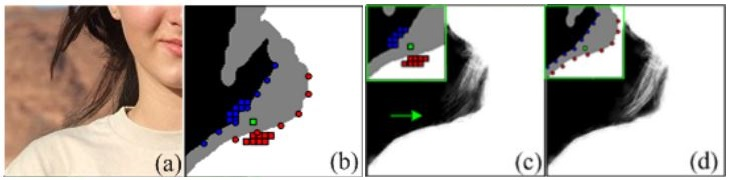
\includegraphics[width=1\columnwidth]{Chapter2/2/robust_figure_1.jpg}
\caption[Robust matting sampling strategy.]{\textit{Optimized colour sampling for robust matting} sampling strategy. Samples are gathered sparsely from the unknown region boundary and densely close to the unknown region. Figure taken from \cite{robust}.}
\label{fig:robust-f1}
\end{figure}

They also proceed to refine the estimated matte by assuming local smoothness, assuming that estimated $\alpha$’s with high confidence are correct and using them in a graph based labelling model.
The algorithm was further refined to a method called \textit{Soft Scissors} \cite{softscissors} that incrementally solved the matte based on user input. The matte is basically solved in real time; the user can brush along a foreground object’s boundary and the resulting alpha values can be viewed. An interesting fact is that the brush size that the user hovers over the image grows depending on the size of the mixed pixel region as seen in Figure \ref{fig:robust-f3}. An overview of the method can be seen in Figure \ref{fig:robust-f2}. 

\begin{figure}[t!]
\centering
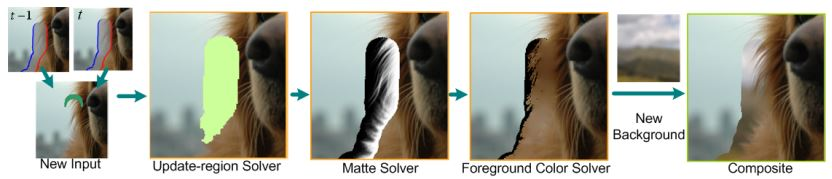
\includegraphics[width=1\columnwidth]{Chapter2/2/robust_figure_2.jpg}
\caption[A flow chart of Soft Scissors workflow.]{A flow chart of \textit{Soft Scissors} workflow. Figure taken from \cite{softscissors}.}
\label{fig:robust-f2}
\end{figure}

\begin{figure}[t!]
\centering
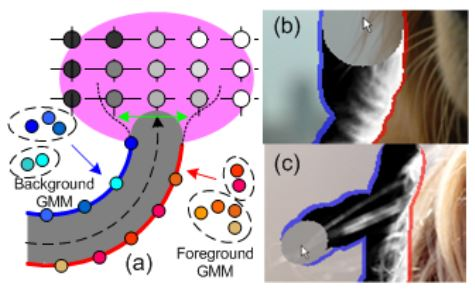
\includegraphics[width=0.7\columnwidth]{Chapter2/2/robust_figure_3.jpg}
\caption[Soft scissors automatic brush width adjustment.]{\textit{Soft scissors} automatic brush width adjustment. Figure taken from \cite{softscissors}.}
\label{fig:robust-f3}
\end{figure}

Another observation made by Gastal and Oliviera \cite{shared}, was that nearby pixels share similar foreground, background and $\alpha$ values and thus extra computation can be avoided, leading to a real time approach. The first step is basically to expand the trimaps’ known regions based on pixel affinities. For the sampling process, spatially close sample pairs are taken as illustrated in Figure 11. Then, the matte is estimated and locally smoothed using a smoothness algorithm.

\begin{figure}[t!]
\centering
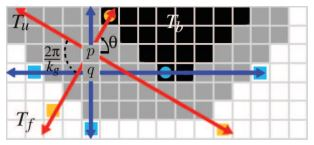
\includegraphics[width=0.6\columnwidth]{Chapter2/2/shared_figure_1.jpg}
\caption[\textit{Shared sampling for real-time alpha matting} sampling strategy.]{In \textit{Shared sampling for real-time alpha matting}, the spatially closest samples are selected. Each unknown pixels sample via different paths. Figure taken from \cite{shared}.}
\label{fig:shared-1}
\end{figure}

%%%%%%%%%%%%%%%%%%%%%%%%%%%%%%%%%%%%%%%%%%%%%%%%%%%%%%%%%%%%%%%%%%%%%%%%
\section{Latest matting methods}
\label{sec:latest-matting-methods}

After multiple methods were proposed to solve the matting problem, algorithms were still struggling to give satisfying results. The problem is that natural images are so variable that it is difficult to formulate a solution that works for every case. So far researches used their own datasets and there were no actual comparisons between methods. So the need for a standardized benchmark dataset led to the creation of a perceptual benchmark website \cite{benchmark} that offered datasets for researchers to use and performance evaluations both metric and visual. The error measures used are \textit{sum of absolute differences} SAD, \textit{mean square error} MSE, a \textit{gradient} measure and a \textit{connectivity} measure. The datasets consist of eight test images that are used for the performance comparisons, and twenty six train images with their respective ground truths that are used for training purposes. All images are provided in high and low resolutions, with variable amounts of transparency in each image and different types of trimaps; with wide unknown regions and with narrow. Since the matting problem was already well formulated but with unsatisfying results, from there on research focused on improving the quality of estimated mattes rather than on new mathematical formulations. In this section some of the state of the art methods for natural image matting are presented.
\par
Most matting algorithms assume pixel affinities either for sampling, for selecting the best foreground and background tuple, or for the alpha matte refinement. In \cite{nonlocal} the authors use the \textit{non-local} principle in an attempt to reduce user effort and provide an improved matting method over other ones that use scribbles instead of a trimap. This method is based on the \textit{non-local means} algorithm that is used for image denoising, in combination with the matting principles from \cite{closedform}. The idea is that instead of using pixels that are neighbouring to a pixel, use a weighted average of pixels that are considered to be the most similar. Figure 12 demonstrates the trimap generation by creating graph clusters and by using sparse user input.

\begin{figure}[t!]
\centering
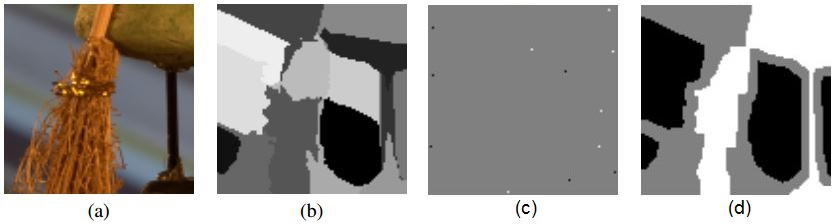
\includegraphics[width=1\columnwidth]{Chapter2/2/nonlocal_figure_1.jpg}
\caption[Non-local matting trimap generation.]{\textit{Non-local matting} trimap generation. Input image (a). Clusters (b). Sparse user input (c). Resulting trimap (d). Figure taken from \cite{nonlocal}.}
\label{fig:nonlocal-1}
\end{figure}

In \textit{KNN matting} \cite{knn} the authors use the idea of non-local matting, but instead of using the colour line model assumption from \cite{closedform}, they use a \textit{k-nearest neighbour} approach and also extract multiple alpha mattes as image layers. Their method uses a \textit{feature vector} (\ref{eq:knn-e1}) to represent pixels and depending on the scenario, different colour spaces are used along with pixel spatial information. In their article, they mention the usage of the HSV colour space with Hue \textit{h}, Saturation \textit{s} and Value \textit{v}. For each pixel in the unknown region the \textit{k-nearest neighbours} are selected (Figure 13) in the feature space using a kernel function defined in (\ref{eq:knn-e2}) and depending on the values of k, the layers of foreground and background can be extracted (Figure 14) and graph clusters can be created for each pixel.

\begin{equation} \label{eq:knn-e1}
X(i)=(cos(h),sin(h),s,v,x,y)_{i}
\end{equation}

\begin{equation} \label{eq:knn-e2}
K(i,j)=1-\frac{\left \| X(i)-X(j) \right \|}{C}
\end{equation}

\begin{figure}[t!]
\centering
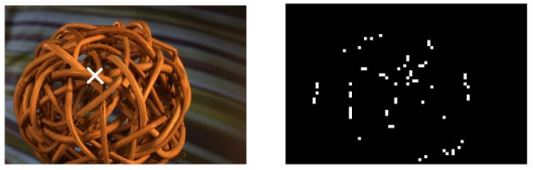
\includegraphics[width=1\columnwidth]{Chapter2/2/knn_figure_1.jpg}
\caption[KNN sampling strategy.]{\textit{KNN matting} sampling strategy. For a selected pixel (left) KNN collects samples (right) using a non-local method. Figure taken from \cite{knn}.}
\label{fig:knn-f1}
\end{figure}

\begin{figure}[t!]
\centering
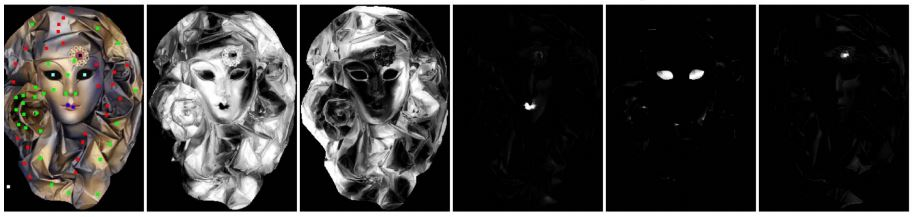
\includegraphics[width=1\columnwidth]{Chapter2/2/knn_figure_2.jpg}
\caption[KNN input clicks for alpha-mask extraction]{\textit{KNN matting} input clicks for alpha-mask extraction. Different input clicks are needed for different mask extraction. Figure taken from \cite{knn}.}
\label{fig:knn-f2}
\end{figure}

\begin{figure}[t!]
\centering
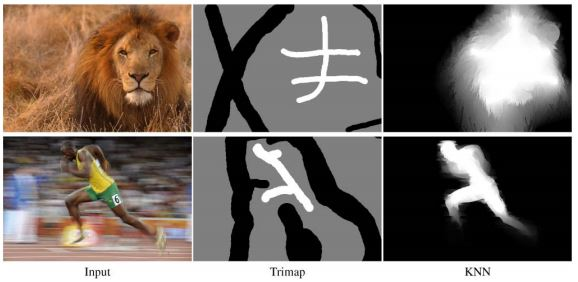
\includegraphics[width=1\columnwidth]{Chapter2/2/knn_figure_3.jpg}
\caption[KNN performance on fuzzy regions.]{\textit{KNN matting} performs poorly on images with a high amount of mixed pixels. Figure taken from \cite{knn}.}
\label{fig:knn-f3}
\end{figure}

A common problem that occurs in natural image matting, is estimating $\alpha$ in the case where foreground and background colour distributions are overlapping. In this case foreground and background regions cannot be distinguished and sampling methods using common colour spaces fail. A method proposed \cite{texture} to tackle this issue was the combination of colour features with \textit{texture features}. The texture feature is a combination of \textit{chromatic} and \textit{structural} content of the image. For the chromatic texture features, the image is smoothed using \textit{bilateral filters} that preserve image edges, and obtain a high, medium and low smoothing of the image. The structural texture feature is obtained through \textit{Haar wavelet decomposition} of the image into four sub images. The feature vector is formulated as:

\begin{equation} \label{eq:texture-e1}
FV_{T}=\{A^{grad}_{(l,c)}, A^{var}_{(l,c)}, A^{mean}_{(l,c)}, H^{mean}_{(l,c)}, V^{mean}_{(l,c)}, D^{mean}_{(l,c)}\},\; c=\{R,G,B\},\; l=1,2
\end{equation}

A high dimension texture feature is produced and is reduced via \textit{principal component analysis} PCA. The same sampling strategy as in \cite{shared} is used. For the classification process, texture is considered using a greater weight when colour feature distributions are overlapping (Figure 16). The alpha matte produced is then refined using an iterative approach.

\begin{figure}[t!]
\centering
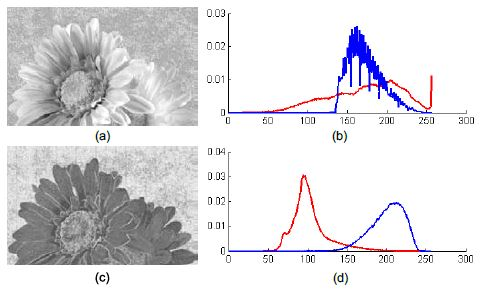
\includegraphics[width=0.8\columnwidth]{Chapter2/2/texture_figure_1.jpg}
\caption[Colour and texture image colour distributions.]{Intensity image with overlapping intensity distributions (top) and texture image with intensity distributions separated (bottom). Figure taken from \cite{texture}.}
\label{fig:texture-f1}
\end{figure}

\begin{figure}[t!]
\centering
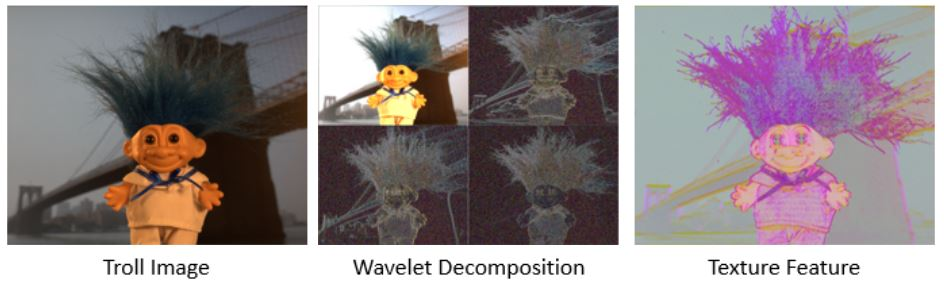
\includegraphics[width=1\columnwidth]{Chapter2/2/texture_figure_2.jpg}
\caption[Haar wavelet decomposition and resulting texture image.]{Visual representation of \textit{Haar wavelet decomposition} and resulting texture image. Figure taken from \cite{texture}.}
\label{fig:texture-f2}
\end{figure}

Another contribution by the same researchers in association with \textit{Adobe Research}, was to solve the problem of sampling non-representative samples. This comprehensive sampling approach \cite{comprehensive}, separates the trimap known region in to sub regions that are activated iteratively for sampling. Basically the more spatially close the samples are, the less the colour variation, and the further away there are the more colour variation is needed. This idea is illustrated in Figure 18. For selection of the best foreground and background sample pair, chromatic distortion \textit{K}, and spatial \textit{S} and colour \textit{C} statistics are considered (\ref{eq:comprehensive_e1}). The matte is further refined using the laplacian proposed in \cite{closedform}.

\begin{equation} \label{eq:comprehensive_e1}
O_{z}(F_{i},B_{i})=K_{z}(F_{i},B_{i})\times S_{z}(F_{i},B_{i})\times C_{z}(F_{i},B_{i})
\end{equation}

\begin{figure}[t!]
\centering
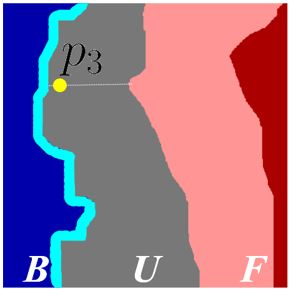
\includegraphics[width=0.4\columnwidth]{Chapter2/2/comprehensive_figure_1.jpg}
\caption[Comprehensive matting sampling strategy.]{\textit{Improving Image Matting Using Comprehensive Sampling Sets} sampling strategy. A pixel in unknown region (grey) samples from the activated foreground region (light blue), and from activated background region (light red). Figure taken from \cite{comprehensive}.}
\label{fig:comprehensive-f1}
\end{figure}

%%%%%%%%%%%%%%%%%%%%%%%%%%%%%%%%%%%%%%%%%%%%%%%%%%%%%%%%%%%%%%%%%%%%%%%%%%%%%%%%%%%55
\section{Extention to video}
\label{sec:extention-to-video}

Since the introduction of the blue screen matting technique, video matting has been increasingly used in the industry. Consequently research has also been focused to extend natural image mating to matting of natural video scenes. The basic challenges in video matting is the large data set, so algorithms must be fast enough to compensate for it, temporal coherence of frames, because the human visual system is sensitive to temporal inconsistencies, and fast motions that cannot be caught by the typical 30 frames per second that cameras capture, that cause motion blur. Because it would be impossible to define trimaps for every single frame manually, typical methods for introducing prior information is to define trimaps in key frames and interpolate the rest, by using \textit{optical flow} algorithms or use hard segmentation algorithms that are temporally consistent. Tracking algorithms that are used in computer vision for background removal, unfortunately cannot be used in matting because results of such methods are too coarse and not accurate enough either to generate a trimap or to give information to be used directly in a matting algorithm.
\par
The first video matting algorithm \cite{video} was based on Bayesian matting \cite{bayesian} and used with optical flow for temporal coherence. Trimaps were created by interpolating between keyframe trimaps provided by the user or automatically generated. Optical flow algorithms are used to estimate pixel motion in a video sequence. Assuming that we have two sequential frames, each pixel in one of the frames can be considered to be coming from a shifted location in the other frame, and the displacement of the pixel is described by a \textit{motion vector} and the set of motion vectors is called \textit{flow field} (Figure 19). Assumptions to be made are that the colour of the pixels is considered to estimate the flow field and a flow field should be spatially coherent. Many optical flow algorithms exist in the literature and for this video matting method an algorithm described in \cite{flow} is used. Sequential video frames are used to model a background using image mosaicking techniques \cite{mosaic} that can be used in cases where the background isn’t static to further refine the trimaps, assuming that the background in the video is roughly planar. Figure 20 illustrates the whole process.

\begin{figure}[t!]
\centering
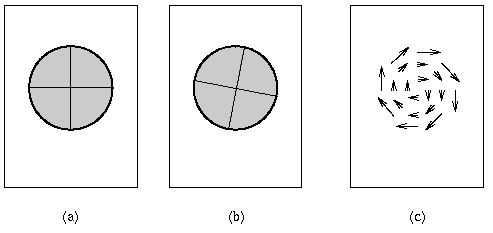
\includegraphics[width=0.8\columnwidth]{Chapter2/2/optical_figure_1.jpg}
\caption[Motion vectors and flow field.]{Two sequential frames at times t (a) and t+1 (b) and the estimated flow field (c). The arrows represent the motion vectors. }
\label{fig:optical-f1}
\end{figure}

\begin{figure}[t!]
\centering
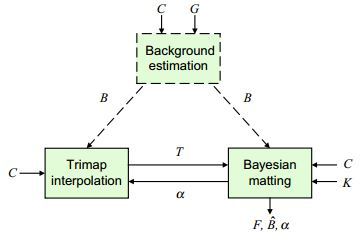
\includegraphics[width=0.8\columnwidth]{Chapter2/2/optical_figure_2.jpg}
\caption[Video matting work-flow.]{Work flow of the video matting algorithm. C is the frame sequence, G is the garbage mattes provided by the user, B is the estimated background, T is the trimap, a is the alpha mattes and K is the user provided keyframe trimaps. Figure taken from \cite{video}.}
\label{fig:optical-f2}
\end{figure}

%%%%%%%%%%%%%%%%%%%%%%%%%%%%%%%%%%%%%%%%%%%%%%%%%%%%%%%%%%%%%%%%%%%%%%%%%%%%%%%%%%%%%%%
\section{Matting with custom hardware}
\label{sec:matting-with-custom-hardware}

Due to the under-constrained nature of the matting problem, user input must be provided in a form of a trimap or sparse scribbles. In video matting, we saw that frame to frame variations can be used as extra information to help with the matting process. Researches have considered in a number of occasions the use of specialized hardware that will provide extra information needed to solve the matting problem.
\par
In \textit{Defocus matting} \cite{defocus}, multiple synchronized video streams are caught using a multi-sensor camera. This camera consists of three components, a pinhole sensor that has a small aperture that creates a large depth of field and is nominally focused on the foreground, a foreground sensor that produces sharp images for objects that are close to the camera and a defocused background, and a background sensor with a large depth of field (Figure 21). A trimap is automatically created by examining the texture of the images, specifically the sharp pixels correspond to the foreground for the foreground focused image and sharp pixels correspond to background for the background focused image. The disadvantages of this method is that the system requires a significant discontinuity between foreground and background and also the system requires stronger illumination than a normal camera.

\begin{figure}[t!]
\centering
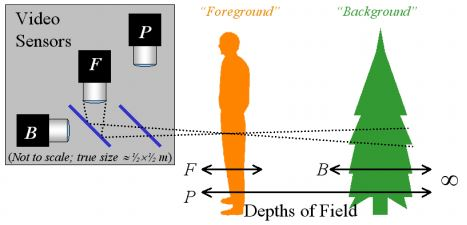
\includegraphics[width=0.9\columnwidth]{Chapter2/2/defocus_figure_1.jpg}
\caption[Defocus matting setup.]{The multi-sensor camera system with a pinhole sensor P, a foreground focused camera F and a background focused camera B. Figure taken from \cite{defocus}.}
\label{fig:defocus-f1}
\end{figure}

In \textit{Flash matting} \cite{flash}, the idea is that when an object is photographed, the flash does not affect the background in a significant way. So if a scene if photographed with and without flash and then the two resulting images are subtracted, the result will be a rough foreground that can be used to produce a trimap. In a sense, this is the reverse process of triangulation \cite{blue}; instead of having two different backgrounds, we have two different foregrounds. The disadvantage of this method is that objects with specular properties may produce an erroneous trimap because the high reflectance areas will not change in the two images.

\begin{figure}[t!]
\centering
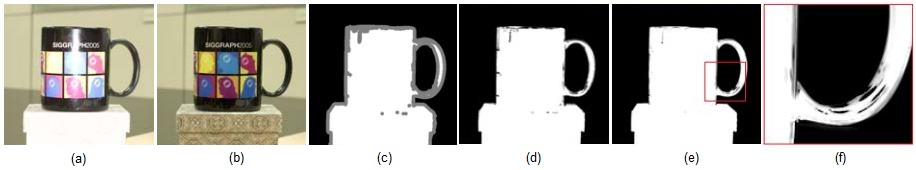
\includegraphics[width=1\columnwidth]{Chapter2/2/flash_figure_1.jpg}
\caption[Flash matting images and results.]{An object photographed with (a) and without (b) flash, the produced trimap (c), and the problematic areas due to specular surfaces. Figure taken from \cite{flash}.}
\label{fig:flash-f1}
\end{figure}

The next approach uses a \textit{camera array} \cite{cameraarray} to solve the matting problem. A synthetic image is created that is focused on the foreground object which reduces the variance of the pixels in the foreground and increases the variance of pixels in the background. The standard matting equation is modified to work with the variances of the images. So basically the foreground is captured in front of multiple backgrounds, created by the parallax of the images. This system has shown good results on a variety of images containing fuzzy and transparent regions and is also quite fast with running times close to real time for VGA images. The drawback though is that the accuracy is limited by aliasing in the light fields and the fact that the system is designed to work better in controlled environments that are usually indoor.
\par
A recent tendency in computer vision is the use of depth information produced by \textit{time of flight} TOF sensors. These sensors are able to produce high quality \textit{depth-maps} that can be further used in the matting process. A depth-map is known to be used for z-buffering in computer graphics, but has many application in computer vision. Extracting depth information from images only is a difficult process, so the use of a device that can provide the depth-map is preferred. In \cite{tof} the authors are using a time of flight sensor in combination with a stereo rig. They first create an initial matte that is extracted from the depth-map produced by the TOF sensor and then the matte and depth are refined. A trimap is created by use of erosion and dilation techniques on the extracted depth and the closed form method \cite{closedform} is used to produce the initial matte. In the refinement phase a cost function is created by using depth, pixel similarity from stereo matching and the confidence from the matte. Figure 23 illustrates the mattes and depth-maps produced.

\begin{figure}[t!]
\centering
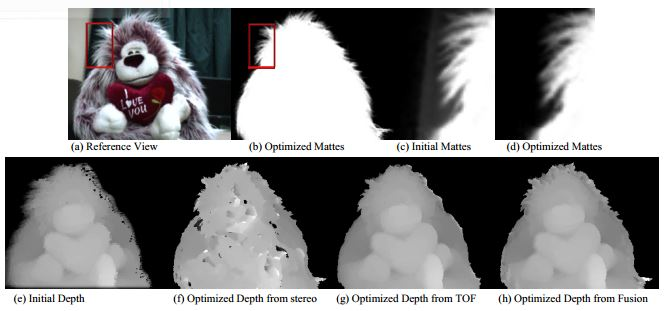
\includegraphics[width=0.8\columnwidth]{Chapter2/2/depth_figure_1.jpg}
\caption[Matting with depth information.]{Estimated alpha matte (b), depth-map (h) and optimizations. Figure taken from \cite{tof}.}
\label{fig:depth-f1}
\end{figure}

An extension of this method in \cite{realtimetof} proposes an automatic real-time video matting system. The system is initialized by using colour and depth information. The hard segmentation is done by modelling foreground, background colours and depth likelihoods and by using \textit{graph cuts}. From the binary mask produced from the hard segmentation, a trimap is generated and refined using the colour and depth information and then the final matte is estimated using multichannel Poisson equations. The algorithm is implemented on GPU and for a low resolution image the hard segmentation implementation can achieve 32fps and the matting implementation archives 80fps. The limitation of this system is that the hard segmentation process is done frame by frame and no temporal coherence is enforced for the trimaps. Figure 24 illustrates the work flow.

\begin{figure}[t!]
\centering
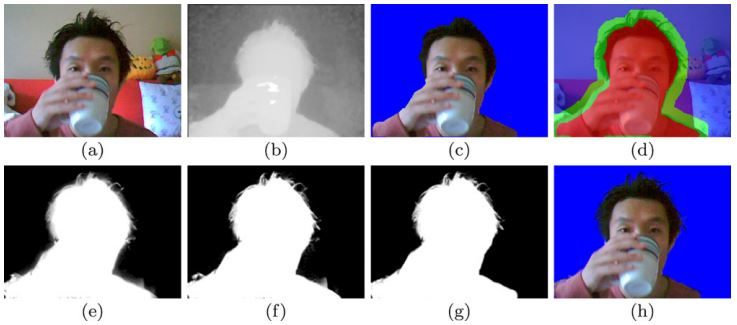
\includegraphics[width=0.8\columnwidth]{Chapter2/2/depth_figure_2.jpg}
\caption[Real-time matting with depth.]{From a colour image (a) and a depth-map (b), a binary mask (c) is produced and refined into a trimap (d). The alpha matte is iteratively produced (e)(f)(g)(h). Figure taken from \cite{realtimetof}.}
\label{fig:depth-f2}
\end{figure}

